%!TEX root = twig-gpu.tex

\section{Code generation}
\label{twig:code-gen}

To generate code, Twig relies on an abstract, language-independent model with a
small number of basic operations. This simplified model is useful for
formulating Twig's semantics, described in Section~\ref{semantics}. It is also
helpful in clarifying the precise operations which Twig supports, without
getting bogged down in the (typically quite complicated) details of outputting
code for a particular programming language.

Twig generates code in units called \emph{blocks}. The term ``block'' is
somewhat overloaded -- our usage differs somewhat from the norm. In Twig, a
block of code represents anything that performs some operation on a set of
inputs, and which produces a set of outputs. Blocks may have zero or more inputs
and outputs. Blocks can also be combined in two different ways:
\emph{sequentially}, or \emph{in parallel}. These operations are described in
more detail below.

Our current implementation of this model supports the generation of C code, and
adds some extra features to support that language. These features include such
details as managing type declarations, support for parameterized blocks, and for
``closing'' blocks, which are generated as variables go out of scope and are
intended to be used to free resources. We are looking into the possibility of
incorporating these and other features into the language-neutral model, but for
the moment they are specific to C.

\begin{figure}[htbp]
\centering
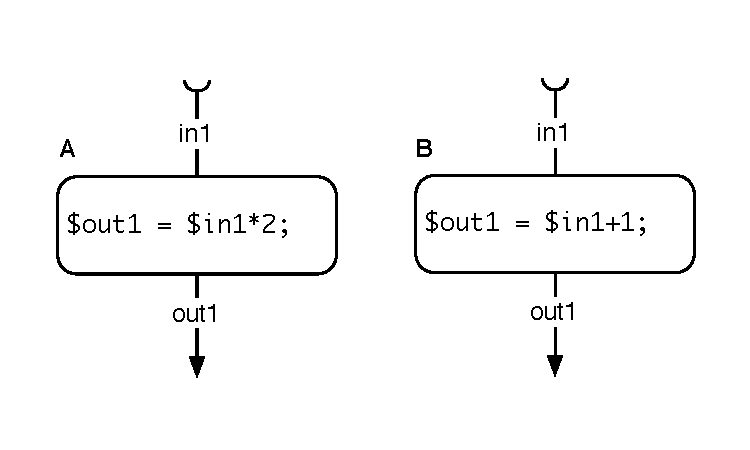
\includegraphics[width=\columnwidth]{images/code-gen1}
\caption{Two basic blocks, A and B.}
\label{fig:codegen-blocks}
\end{figure}

\subsection{Block Composition}

As mentioned above, Twig provides two fundamental binary operations on blocks.
The first is the \emph{sequential composition} operator, represented by the
addition symbol ($+$). Sequencing connects two blocks of code by ``wiring'' the
outputs of the first block into the inputs of the second. In C, this is done by
creating temporary variables which are substituted into the original blocks. For
example, see Figure~\ref{fig:codegen-seq}, which builds on
Figure~\ref{fig:codegen-blocks}.

\begin{figure}[htbp]
\centering
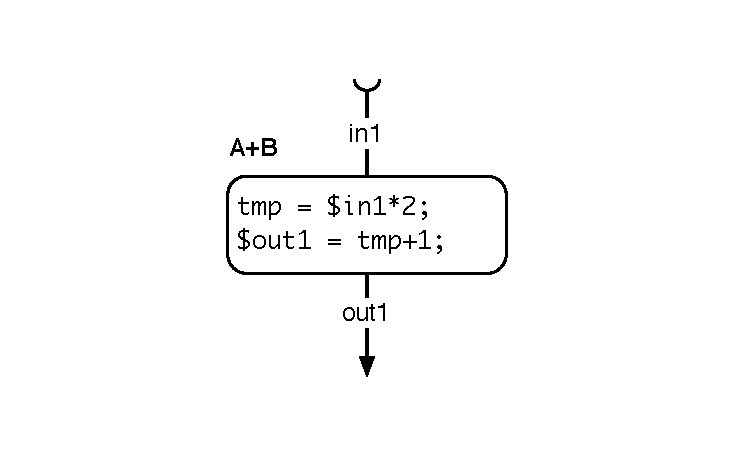
\includegraphics[width=\columnwidth]{images/code-gen2}
\caption{Two blocks from Figure~\ref{fig:codegen-blocks} composed sequentially.
The variable ``tmp'' is created, and renaming performed, so that the output of
block A would flow to the input of block B.}
\label{fig:codegen-seq}
\end{figure}

Twig's implementation for C takes care of declaring and uniquely naming
temporary variables to accomplish sequencing.

The second operator is \emph{parallel composition}. Under this operator, two
blocks are combined so as to execute independently of one another, but to appear
as one single block. We represent this operation with the multiplication
operator ($\times$). An example is shown in Figure~\ref{fig:codegen-par}.

\begin{figure}[htbp]
\centering
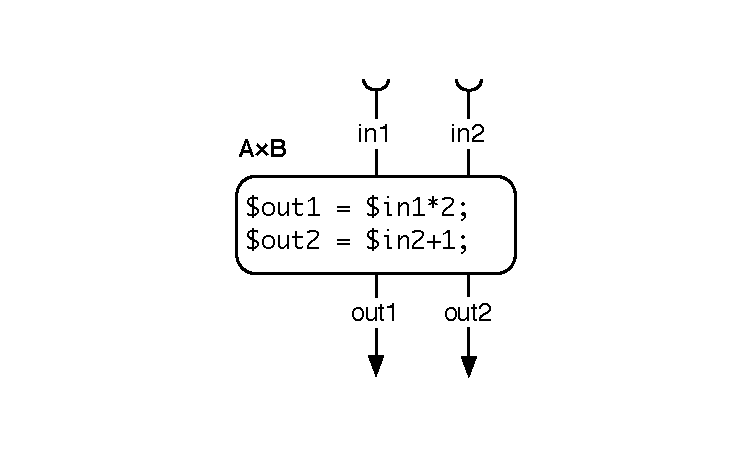
\includegraphics[width=\columnwidth]{images/code-gen3}
\caption{Two blocks from Figure~\ref{fig:codegen-blocks} composed in parallel.
Renaming is performed such that the composed block has two inputs and two 
outputs.}
\label{fig:codegen-par}
\end{figure}

\subsection{Special Blocks}

Twig defines a special set of blocks called \emph{permutation} blocks. These
blocks have some special properties, which we will exploit for the purposes of
rewriting programs to remove redundant memory copies. In particular, some kinds
of blocks act as a kind of identity element when composed with others.

The permutation blocks are referred to as $\Pi_m(i_1,\ldots,i_n)$, and represent
the primitive operation of rearranging $m$ inputs to $n$ outputs, possibly in a
different order, and possibly duplicating or dropping elements. The data is only
passed through, and are otherwise unchanged.

Among the permutation blocks, there are a set of elements for which we provide
special rules; namely, a set of \emph{identity} permutations. The simplest of
these is $\Pi_1(1)$, which acts as an identity transformation with one input and
one output. We refer to this element as $I_1$. In fact, there are an unlimited
number of identity transformations, which take $n$ inputs to $n$ outputs,
unchanged. These are referred to as $I_n$, where $1 \leq n$, and $I_n =
\Pi_n(1,2,\ldots,n)$. The blocks $I_n$ are left- and right-identity elements
under a sequence operation. We sometimes use $I_n$ as a kind of ``no-op.''

Using this simple system, a wide variety of code can be generated.
